\section{Experiments}\label{results}

In this section, we demonstrate the effectiveness of the algorithm presented in Section 2.3 in the context of movement primitive learning for optimally striking motions. We consider two hitting tasks: putting in golf and returning the ball with the racket in table tennis. In each task trajectories and the movement primitives are assigned in joint space. 
% underactuated swing-up belongs to putting-like dynamics problems?

\subsection{Putting}

Putting is a simple and natural domain for ILC algorithms, because it allows a robot to apply ILC to control few degrees of freedom (typically the end joint) while having the dynamics of the other joints act as disturbances. This kind of learning can act as a scalable interface to more complex hitting tasks in the full-joint space.

\subsection{Table Tennis}

As a second and more complex task, we consider table tennis where we are interested in generating and executing accurate ball-hitting motions. The racket is mounted on the end-effector of the 7 degree of freedom (DoF) WAM Barrett arm as can be seen in Figure~\ref{barrettArm}. A fixed ball-thrower is available to throw balls accurately to a fixed position in cartesian space, using which 7 joint-space reference trajectories are calculated. These trajectories guide the robot to the desired racket position and orientation so that the incoming ball will be hit precisely at the desired time and position with the desired velocity. 

\begin{figure}
\center
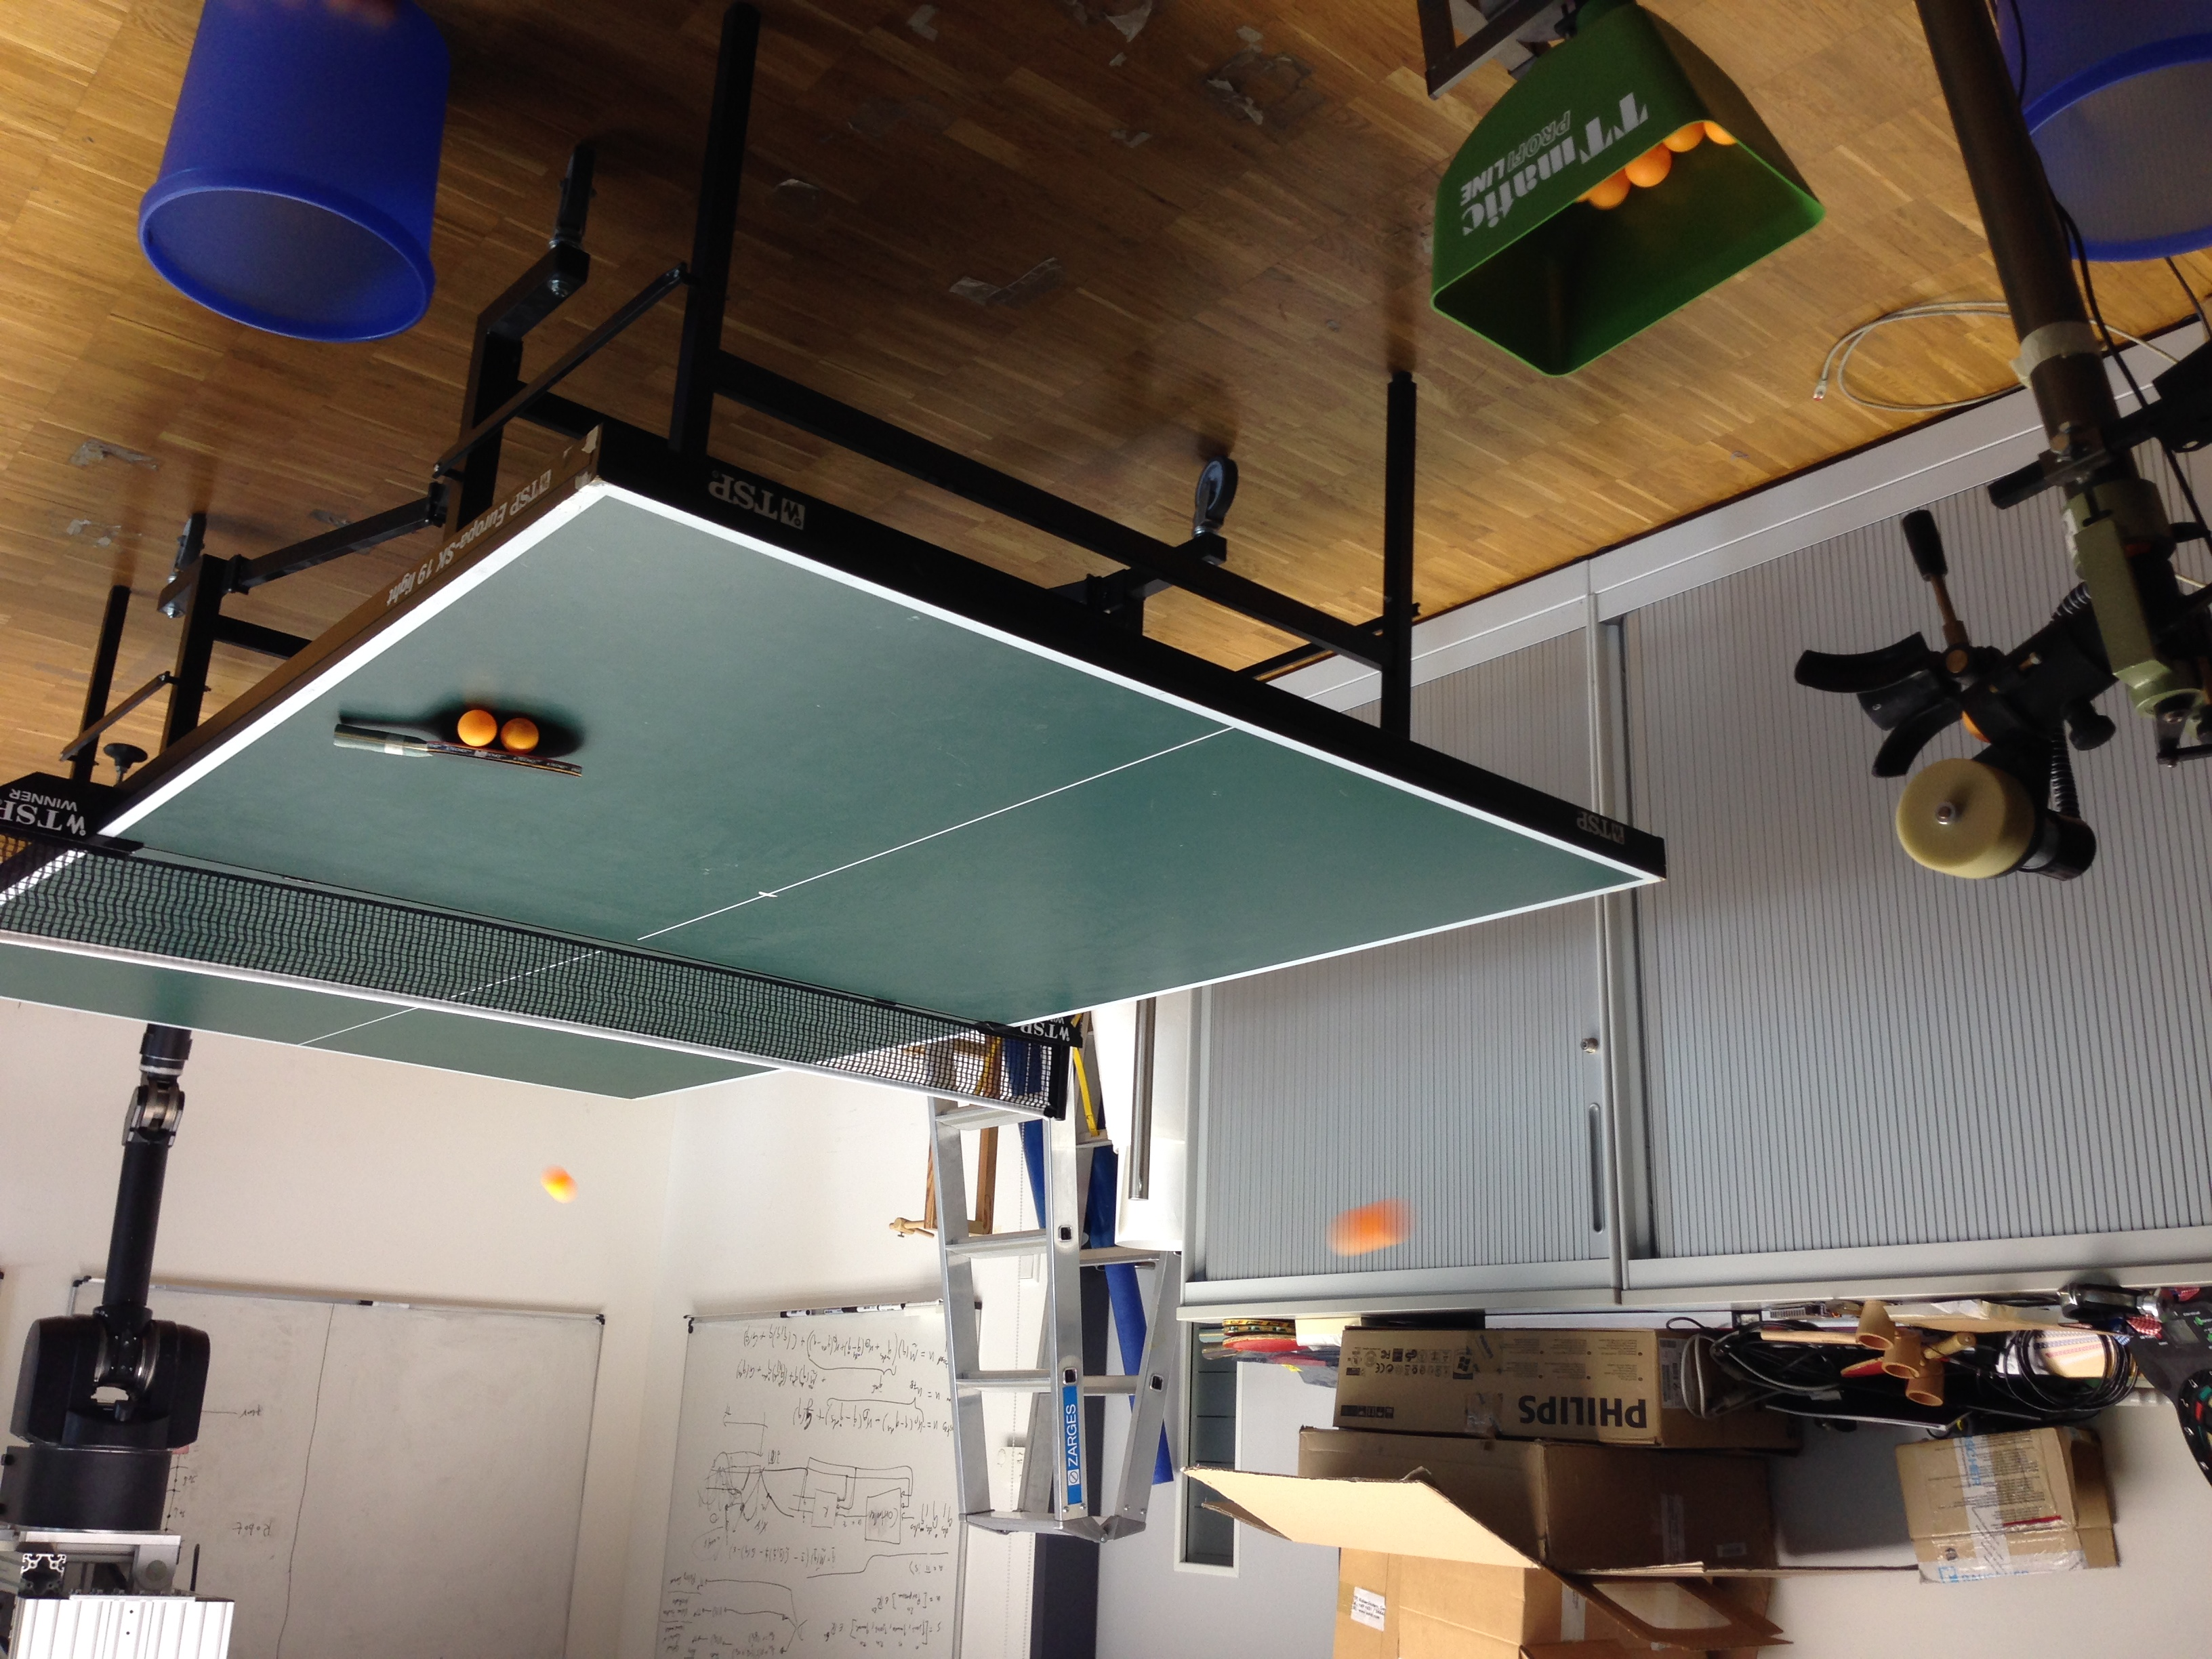
\includegraphics[scale=0.05, angle= 180]{ballgun.jpg}			
\caption{Robotic table tennis setup with the ballgun throwing balls to the robot}
\label{barrettArm}
\end{figure}

The attached video shows the improvement achieved after using $\alg$. The convergence of the algorithm can be seen in Figure 2 and some examples of the generated trajectories in the joint are given in Figure 3. Comparisons to episodic-RL algorithms REPS and PI2 show the advantages, especially the speed and accuracy of the proposed method over them.